
\documentclass[9pt, usenames,dvipsnames]{beamer}

% contains the complete preamble
\usepackage{present}
\usepackage{custom_underline}


\definecolor{preorange}{RGB}{229,129,79}
\definecolor{pregreen}{RGB}{196,202,52}
	         		               		
\title{}
\author[Felix Z.~Hoffmann]{Felix Z.~Hoffmann}
\institute{}
\date{\today}     


\begin{document}


\begin{frame}
  % 
  \vspace{0.6cm}
  
  \begin{center} 
    \huge Modelling the nonrandom and dynamic structure of local
    cortical circuits
  \end{center}
  
  \vspace{1.1cm}

  \large
  \begin{columns}[t]
    %%%% 
    \hfill\Large
    \begin{column}{0.4\textwidth}
      \minipage[c][0.2\textheight][s]{\columnwidth}
      %
      \hspace{0.6cm} Felix Z.~Hoffmann \textcolor{white}{y}
      %
      \endminipage                 
    \end{column}
    %%%% 
    \begin{column}{0.4\textwidth}
      \minipage[c][0.2\textheight][s]{\columnwidth}
      %
      \hspace{0.6cm} Slides: \href{http://bit.ly/bx18s}{bit.ly/bx18s}
      %
      \endminipage           
    \end{column}
    \hfill
    %%%% 
  \end{columns}

  \vspace{-0.3cm}


  \begin{center}
    \Large Bernstein Conference 2018 Satellite Workshop:\\
    \textit{Adaptivity and Inhomogeneity in Neuronal Networks}
  \end{center}

  \bigskip
  \medskip

  \vspace{0.5cm}
  
  \begin{figure}
    \centering
    
\includegraphics[width=\textwidth]{%
      img/logo_banner3.png} %
  \end{figure}



\end{frame}




%% Intro
\begin{frame}{The dynamic connectome}

  \begin{columns}
    % 
    \begin{column}{.85\textwidth}

      
      \begin{figure}
        \hfill
        \includegraphics<1>[width=0.95\textwidth]{%
          figures/Loewenstein2015_Fig1A.png} %
      \end{figure}
      

    \end{column}
    % 
    \begin{column}{.15\textwidth}
      \minipage[c][0.65\textheight][s]{\columnwidth}
      \LARGE
      \vspace{2.3cm}
      Day 0

      \vspace{1.4cm}
      Day 4        
      \endminipage              
    \end{column}
  \end{columns}
  



  \pnote{
    
    - chronic two-photon imaging through\\
    a cranial window
    
    - auditory cortex in mice (expressing GFP\\
    in a subset of pyramidal neurons)

    Figure: 4 Days apart!

    - image spines from 8 neurons\\
    spine count almost constant!
    
    
  }

  
  \source{\cite{Loewenstein2015}}

  
\end{frame}


\begin{frame}{Robust nonrandom connectivity patterns}
  % 
  \begin{columns}
    % 
    \begin{column}{.45\textwidth}
      \minipage[c][0.75\textheight][s]{\columnwidth}
      
      \begin{figure}
        \centering
        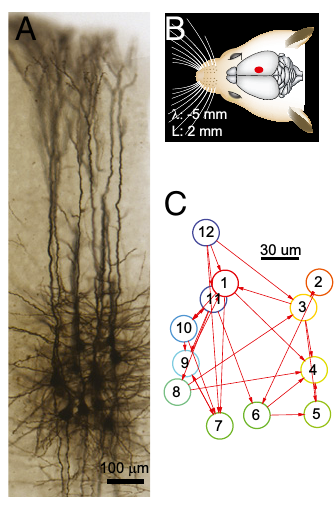
\includegraphics[width=\textwidth]{%
          figures/Perin2011_Fig1ABC.png} %
      \end{figure}
      

      
      \endminipage      
    \end{column}
    % 
    \begin{column}{.55\textwidth}
      \onslide<2->

      \vspace{-0.2cm}
      
      \begin{figure}
        \centering
        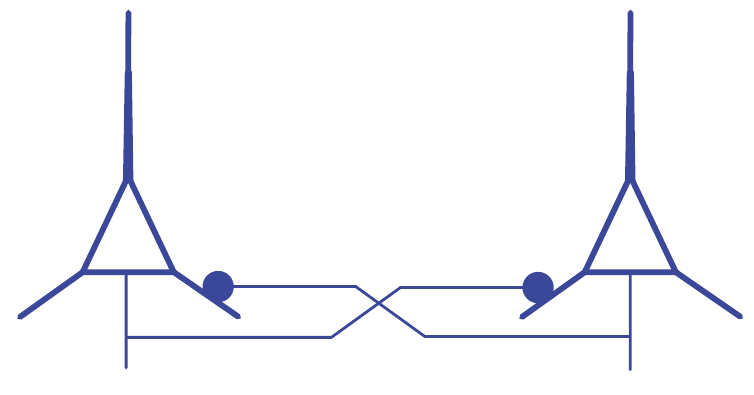
\includegraphics[width=0.525\textwidth]{%
          figures/two_neuron.png} %
      \end{figure}

      \vfill
      
      \onslide<3->
      \begin{figure}
        \centering
        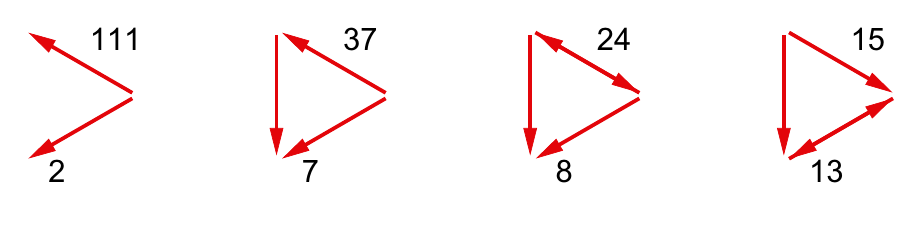
\includegraphics[width=\textwidth]{%
          figures/Perin2011_FigS2_custom.png} %
      \end{figure}

      \vfill
      
      \onslide<4->
      \begin{figure}
        \centering
        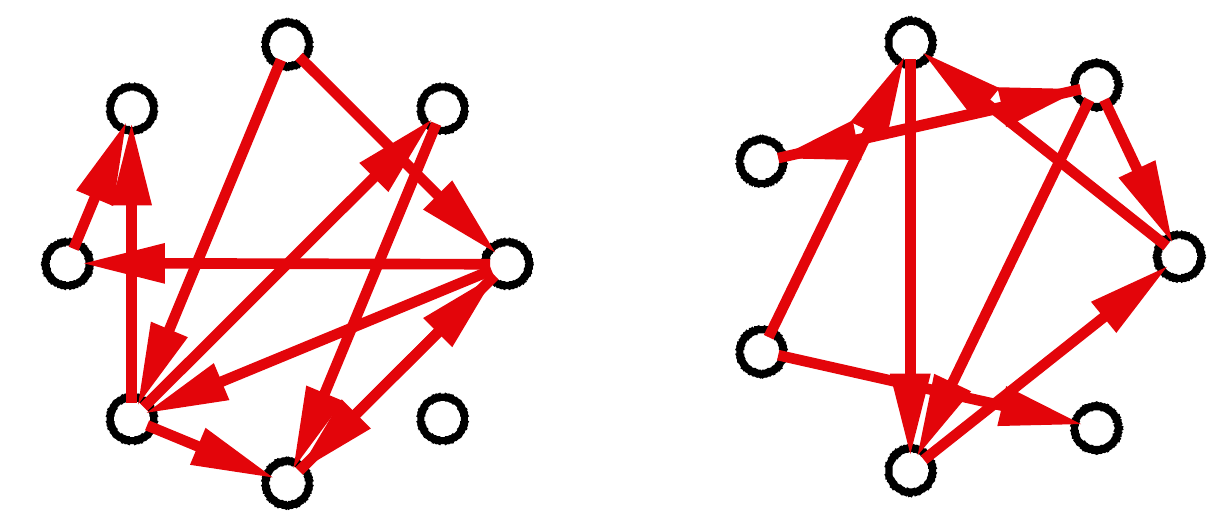
\includegraphics[width=0.7\textwidth]{%
          figures/clust_all.png} %
      \end{figure}
      
      \vfill

      
    \end{column}
  \end{columns}

  \source{\cite{Perin2011, Song2005, Markram1997, Miner2016, Gal2017,
      Vegue2017}}

  \pnote{
    
    These nonrandom structures are well established \\
    and have been reported both experimentally and  \\
    discussed theoretically, but it's interesting to \\
    think about these structures in the light of an \\
    everchanging and quickly rapidly connectome.
    
  }
  
\end{frame}
\begin{frame}{}
  
  
  
\end{frame}



\begin{frame}{Anisotropy in stereotypical axon morphology}

  \only<1>{
    \begin{figure}
      \centering
      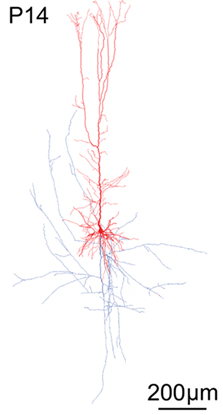
\includegraphics[height=0.75\textwidth]{%
        figures/Romand2011_P14_1.png} 
    \end{figure}}

  \only<2>{\vspace{0.5cm}
    \begin{figure}
      \centering
      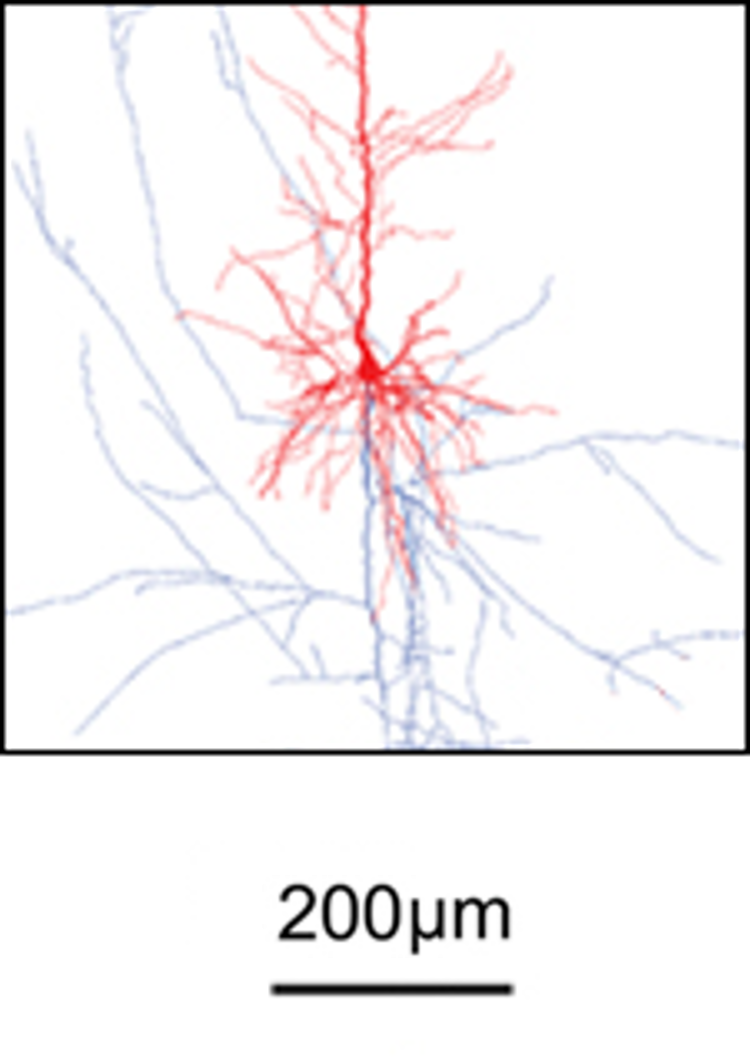
\includegraphics[height=0.7\textwidth]{%
        figures/Romand2011_P14_2.png} 
    \end{figure}}

  \source{%
    \only<1>{\cite{Romand2011}}%
    \only<2>{\cite{Romand2011,Stepanyants2005}}%
  }
  
\end{frame}



%% Model
\begin{frame}{Anisotropic network model}

  % 
  \begin{columns}
    % 
    \begin{column}{.5\textwidth}
      \minipage[c][0.65\textheight][s]{\columnwidth}

      \begin{center}

        \only<1>{\begin{overpic}[height=0.6\textheight]{%
              figures/aniso_model_0.png}
          \end{overpic}}

        \only<2>{\begin{overpic}[height=0.6\textheight]{%
              figures/aniso_model_1.png}
          \end{overpic}}

        \only<3>{\begin{overpic}[height=0.6\textheight]{%
              figures/aniso_model_2.png}
          \end{overpic}}

        \only<4>{\begin{overpic}[height=0.6\textheight]{%
              figures/aniso_model_3.png}
            \put(34.9,50.5){\fboxsep=3pt\colorbox{white}{\LARGE$\alpha$}}
          \end{overpic}}

        \only<5>{\begin{overpic}[height=0.6\textheight]{%
              figures/aniso_model_4.png}
            \put(41,44.5){\Large $\frac{w}{2}$}
            \put(31.9,37.5){\Large $\frac{w}{2}$}
          \end{overpic}}

        \only<6>{\begin{overpic}[height=0.6\textheight]{%
              figures/aniso_model_5.png}
          \end{overpic}}

        
      \end{center}
      
      \endminipage      

    \end{column}
    % 
    \begin{column}{.5\textwidth}
      \minipage[c][0.65\textheight][s]{\columnwidth}
      \large
      \vspace{0.25cm}
      \onslide<1->
      Distribute $N=1000$ neurons randomly on a square surface

      \vfill
      \onslide<3->
      For each neuron\\[-0.2cm]

      \begin{itemize}[leftmargin=0.5cm]

        \itemsep8pt
        
       \item<4->[-] assign a random angle $\alpha$ 

       \item<5->[-] find targets within distance $w/2$ of
         $\alpha$-projection

       \item<6->[-] connect to targets
         
      \end{itemize}
     
      \vspace{1.05cm}
      
      \endminipage      
    \end{column}
  \end{columns}

  \source{Hoffmann \& Rotter, in prep.}

\end{frame}


\begin{frame}{Anisotropic network model}
  % 
  \begin{columns}
    % 
    \begin{column}{.5\textwidth}

      \begin{center}

      \begin{overpic}[width=0.425\textwidth]{%
          targets/012.png}
      \end{overpic} \hspace{0.1cm}
      \begin{overpic}[width=0.425\textwidth]{%
          targets/024.png}
      \end{overpic}

      \begin{overpic}[width=0.425\textwidth]{%
          targets/090.png}
      \end{overpic} \hspace{0.1cm}
      \begin{overpic}[width=0.425\textwidth]{%
          targets/037.png}
      \end{overpic}

      \begin{overpic}[width=0.425\textwidth]{%
          targets/069.png}
      \end{overpic} \hspace{0.1cm}
      \begin{overpic}[width=0.425\textwidth]{%
          targets/061.png}
      \end{overpic}

      \end{center}

      \begin{center}
        targets
      \end{center}
      
    \end{column}
    % 
    \begin{column}{.5\textwidth}


      \begin{center}
        
      \begin{overpic}[width=0.425\textwidth]{%
          inputs/053.png}
      \end{overpic} \hspace{0.1cm}
      \begin{overpic}[width=0.425\textwidth]{%
          inputs/035.png}
      \end{overpic}

      \begin{overpic}[width=0.425\textwidth]{%
          inputs/019.png}
      \end{overpic} \hspace{0.1cm}
      \begin{overpic}[width=0.425\textwidth]{%
          inputs/024.png}
      \end{overpic}

      \begin{overpic}[width=0.425\textwidth]{%
          inputs/091.png}
      \end{overpic} \hspace{0.1cm}
      \begin{overpic}[width=0.425\textwidth]{%
          inputs/018.png}
      \end{overpic}

    \end{center}

      \begin{center}
        inputs
      \end{center}

      
    \end{column}
  \end{columns}

\end{frame}


% \begin{frame}{Anisotropic network model -- Distance-dependency}

%   \begin{figure}
%     \centering \includegraphics<1>[width=1.1\textwidth]{%
%       /home/fh/sci/lab/aniso_netw/ploscb_18/fig/slides/fig3C_2n_dstprf_wfit.png} %
%     \includegraphics<2>[width=1.1\textwidth]{%
%       /home/fh/sci/lab/aniso_netw/ploscb_18/fig/slides/fig3C_2n_dstprf_wfit_data.png} %
%   \end{figure}
  
  
% \end{frame}



%% Results

\begin{frame}{Distance-dependent connectivity in anisotropic networks}
  % 
  \begin{columns}
    % 
    \begin{column}{.45\textwidth}
      \begin{figure}
        \centering
        \includegraphics[width=0.85\textwidth]{%
          figures/netw_dist-dep_aniso.pdf} %
      \end{figure}


    \end{column}
    % 
    \begin{column}{.55\textwidth}
      \begin{figure}
        \centering
        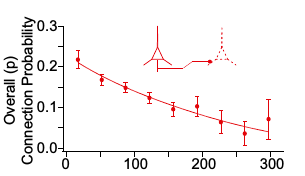
\includegraphics[width=\textwidth]{%
          figures/Perin2011_Fig1E.png} %
      \end{figure}

      
    \end{column}
  \end{columns}

  \vspace{0.95cm}

  \Large
  \begin{columns}
    % 
    \begin{column}{.45\textwidth}
      \minipage[c][0.15\textheight][s]{\columnwidth}
      \begin{center}
        anisotropic network
      \end{center}

      
      
      \endminipage      
    \end{column}
    % 
    \begin{column}{.55\textwidth}
      \minipage[c][0.15\textheight][s]{\columnwidth}
      \begin{center}
        somatosensory cortex\\ \textcite{Perin2011}
      \end{center}
            
      \endminipage           
    \end{column}
  \end{columns}

  
\end{frame}



\begin{frame}{Tuned anisotropic network}
  %
  \vspace{-0.8cm}
  \begin{columns}
    % 
    \begin{column}{.5\textwidth}
      \minipage[c][0.45\textheight][s]{\columnwidth}

      \begin{figure}
        \centering
        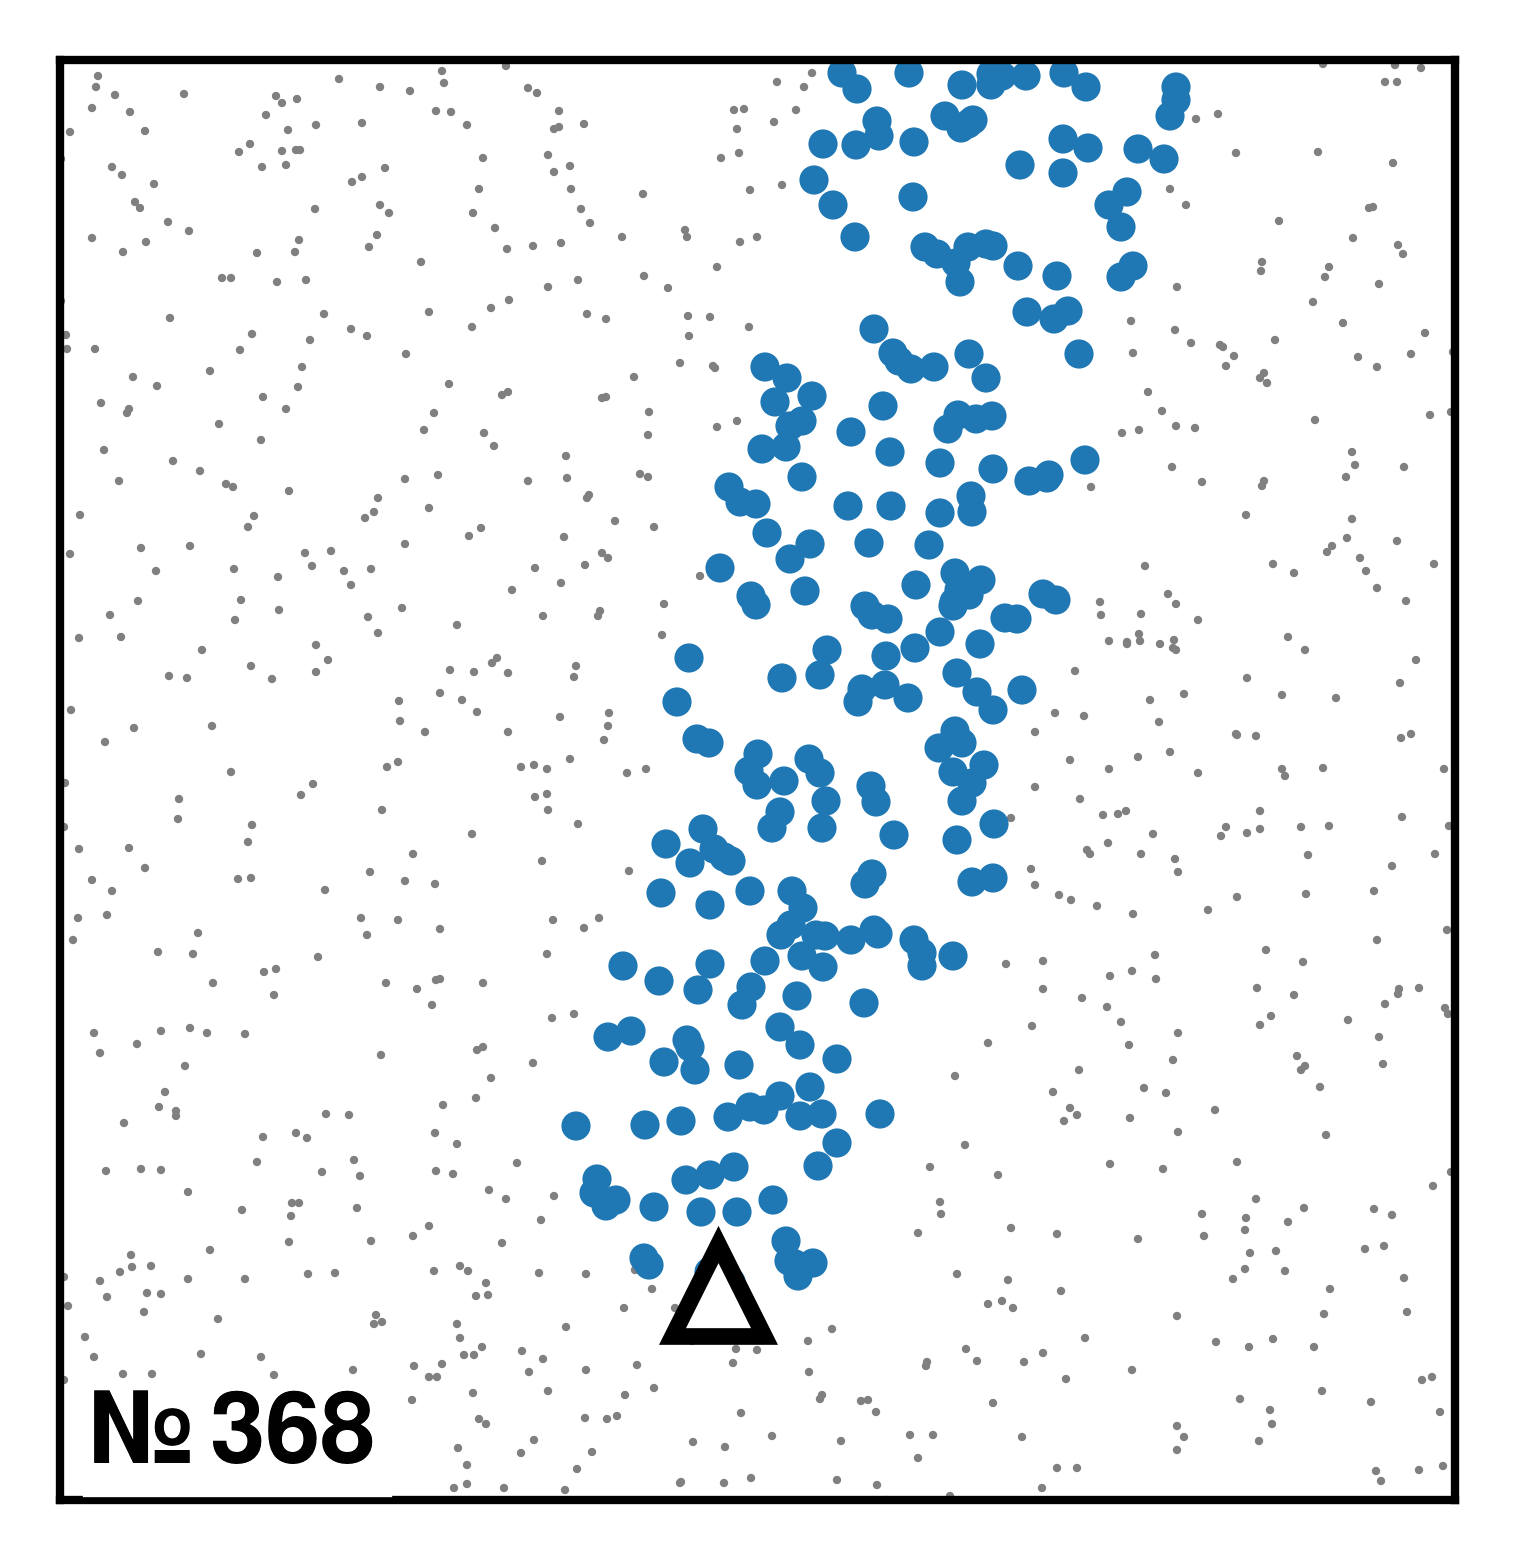
\includegraphics[width=0.65\textwidth]{%
          figures/aniso_netw_targets.png} %
      \end{figure}
      
      
      \endminipage      
    \end{column}
    % 
    \begin{column}{.5\textwidth}
      \minipage[c][0.45\textheight][s]{\columnwidth}

      \begin{figure}
        \centering
        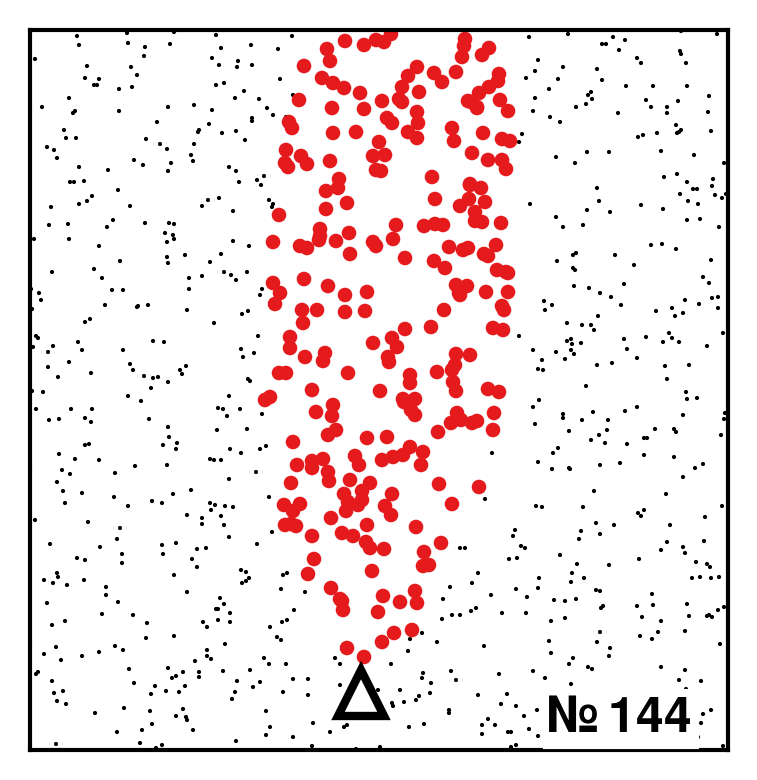
\includegraphics[width=0.65\textwidth]{%
          figures/tuned_aniso_netw_targets.png} %
      \end{figure}
      
      \endminipage
    \end{column}
  \end{columns}

  \vspace{-0.6cm}
  
  \begin{columns}
    % 
    \begin{column}{.5\textwidth}
      \minipage[c][0.25\textheight][s]{\columnwidth}

      \begin{figure}
        \centering
        \includegraphics[width=0.8\textwidth]{%
          figures/netw_dist-dep_aniso.pdf} %
      \end{figure}

      
      
      \endminipage      
    \end{column}
    % 
    \begin{column}{.5\textwidth}
      \minipage[c][0.25\textheight][s]{\columnwidth}

      \begin{figure}
        \centering
        \includegraphics[width=0.8\textwidth]{%
          figures/fig2H_tuned-aniso-ddcp.png} %
      \end{figure}

      
      
      \endminipage      
      
      
    \end{column}
  \end{columns}
  


  
\end{frame}







\begin{frame}{Results -- Overrepresentation of reciprocal connections}

  \begin{figure}
    \centering
    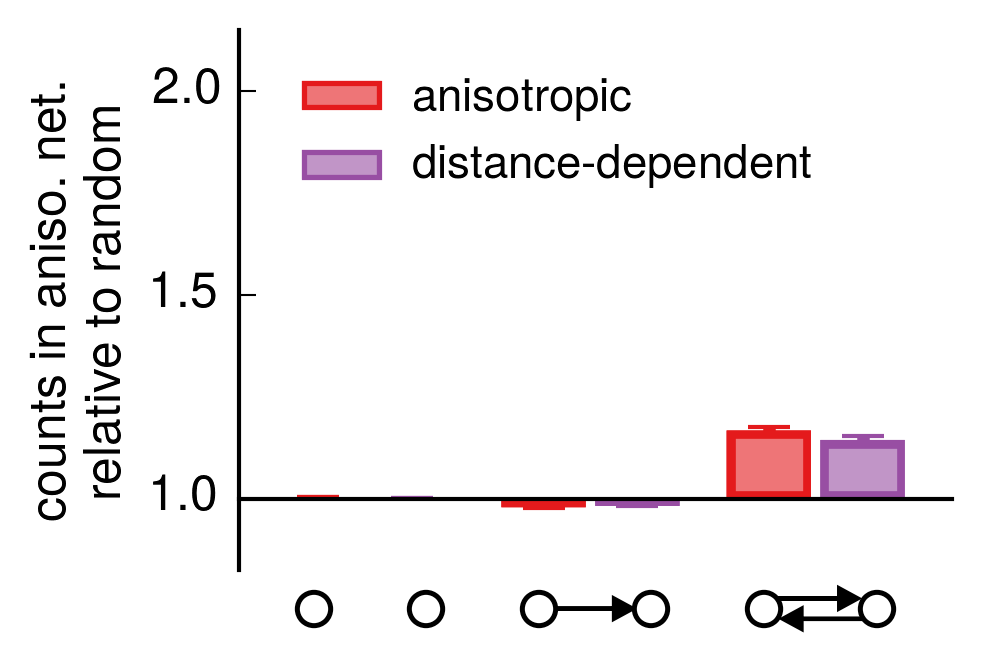
\includegraphics[width=0.78\textwidth]{%
      figures/fig3A_2n_rel_rand.png} %
  \end{figure}
  
  % \source{Hoffmann \& Rotter, in prep.}
  
  
\end{frame}





\begin{frame}{Rewiring anisotropic networks}
  %
  \vspace{-0.8cm}
  \begin{columns}
    % 
    \begin{column}{.5\textwidth}
      \minipage[c][0.45\textheight][s]{\columnwidth}

      \begin{figure}
        \centering
        \includegraphics<1-3>[width=0.925\textwidth]{%
          figures/fig2AD_network_1cell_targets_158-aniso.png} %
        \includegraphics<4->[width=0.925\textwidth]{%
          figures/fig2AD_network_1cell_targets_158-rew.png} %
      \end{figure}
      
      
      
      \endminipage      
    \end{column}
    % 
    \begin{column}{.5\textwidth}
      \minipage[c][0.45\textheight][s]{\columnwidth}

      \vspace{0.2cm}
      
      \begin{center}
      \only<2>{\begin{overpic}[width=0.87\textwidth, frame=1pt]{%
            figures/figE.pdf}
      \end{overpic}}
      \only<3-4>{\begin{overpic}[width=0.87\textwidth, frame=1pt]{%
            figures/figF.pdf}
        \end{overpic}}

      \only<5>{\vspace{0.5cm}\begin{overpic}[width=\textwidth]{%
            figures/netw_dist-dep_aniso-rew.pdf}
        \end{overpic}}      

      \end{center}
      
      \endminipage
    \end{column}
  \end{columns}

  % \vspace{-0.6cm}
  
  % \begin{columns}
  %   % 
  %   \begin{column}{.5\textwidth}
  %     \minipage[c][0.25\textheight][s]{\columnwidth}

  %     \begin{figure}
  %       \centering
  %       \includegraphics[width=0.8\textwidth]{%
  %         figures/netw_dist-dep_aniso.pdf} %
  %     \end{figure}

      
      
  %     \endminipage      
  %   \end{column}
  %   % 
  %   \begin{column}{.5\textwidth}
  %     \minipage[c][0.25\textheight][s]{\columnwidth}

  %     \begin{figure}
  %       \centering
  %       \includegraphics[width=0.8\textwidth]{%
  %         figures/fig2H_tuned-aniso-ddcp.png} %
  %     \end{figure}

      
      
  %     \endminipage      
      
      
  %   \end{column}
  % \end{columns}
  


  
\end{frame}






\begin{frame}{Results -- Overrepresentation of reciprocal connections}

  \only<1>{
  \begin{figure}
    \centering
    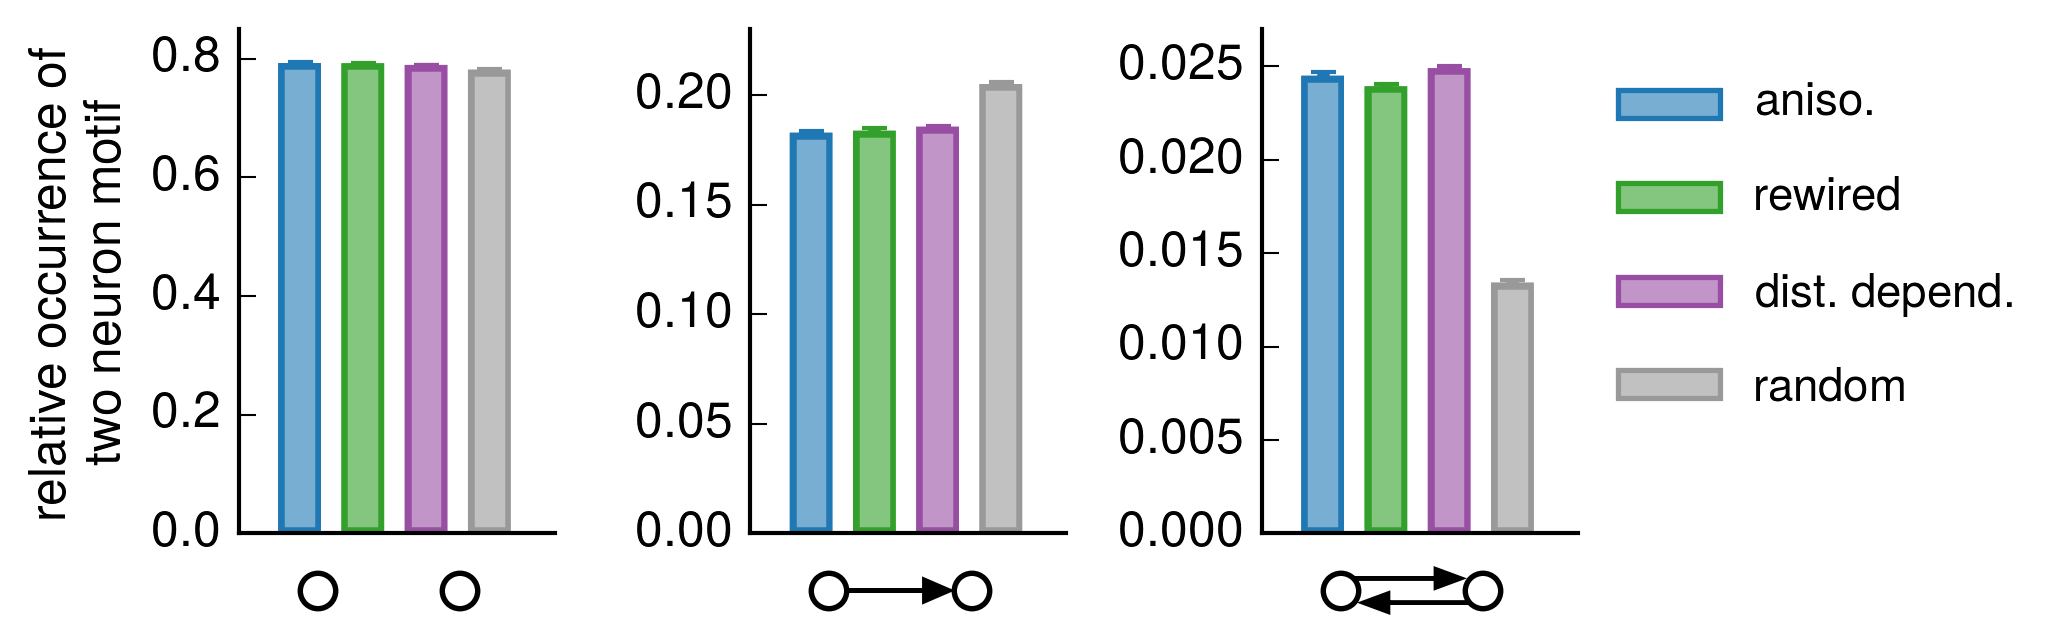
\includegraphics[width=1.07\textwidth]{%
      figures/fig3B_2n_rel_occurrence.png} %
  \end{figure}}


  \only<2>{
  \begin{figure}
    \centering
    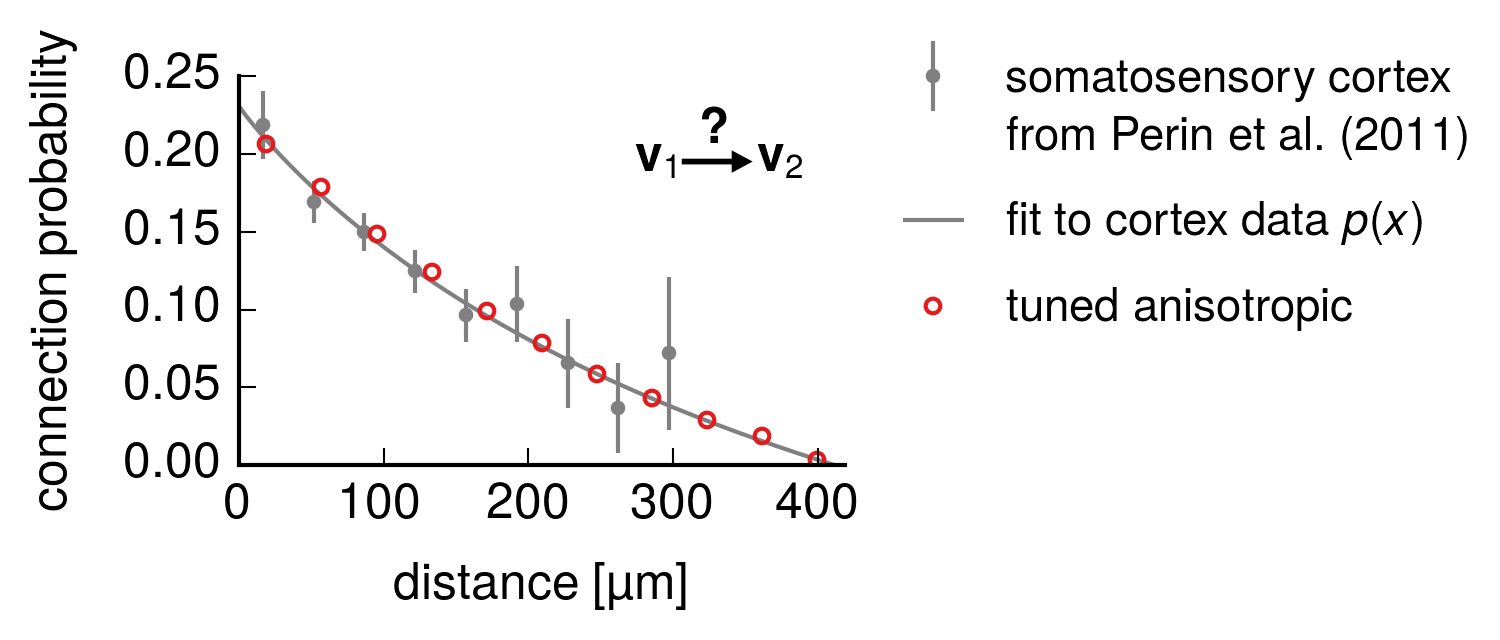
\includegraphics[width=0.88\textwidth]{%
      figures/fig3C_2n_dstprf.png}\\ %
    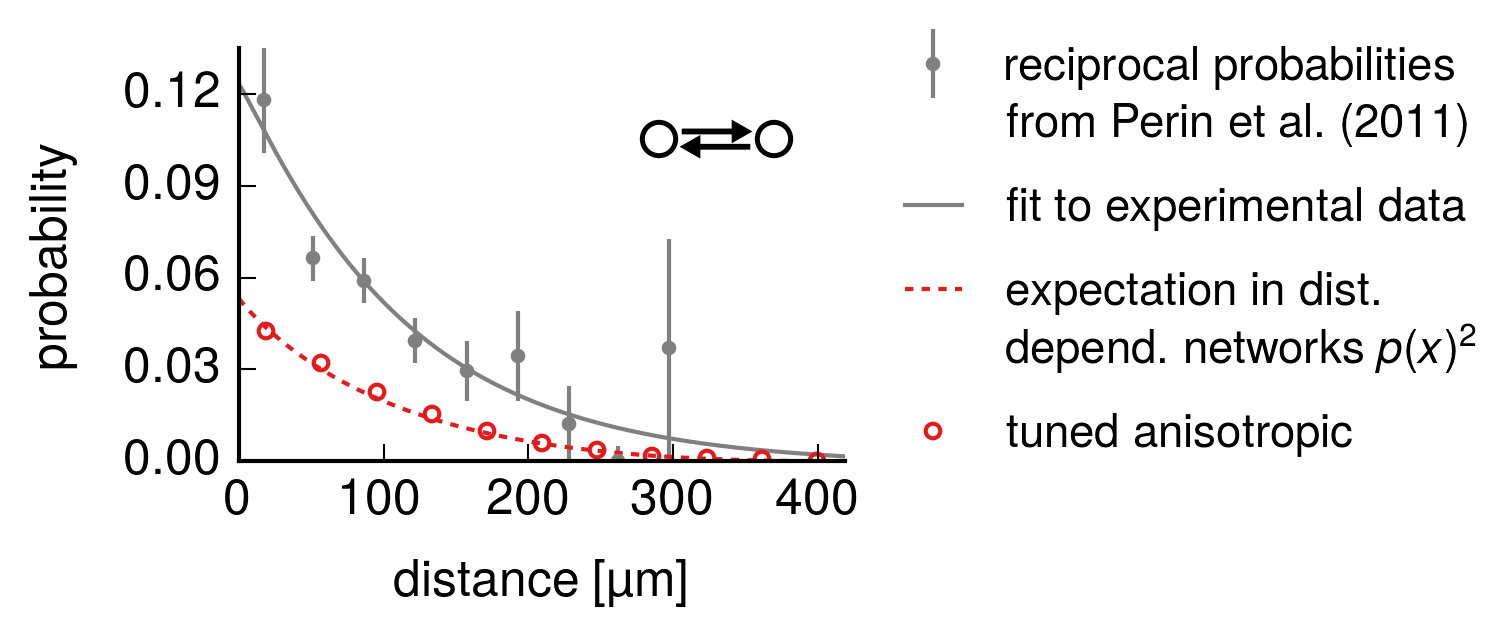
\includegraphics[width=0.88\textwidth]{%
      figures/fig3D_recip_dist.png} %    
  \end{figure}}
  
  % \source{Hoffmann \& Rotter, in prep.}
  
  
\end{frame}





\begin{frame}{}

  \setlength{\parindent}{0pt}

  \vspace{-0.2cm}
  %% \begin{tabular}{ | p{0.44\textwidth}  | p{0.001\textwidth} | p{0.44\textwidth} |}
      \begin{tabular}{  p{0.43\textwidth}   p{0.02\textwidth}  p{0.43\textwidth} }

\onslide<1->{\only<1-7>{
    \begin{center}
      \mbox{\myul{\textit{\textbf{Standard random network model}}}}
    \end{center}}}       

    &&
    \onslide<4->{
    \begin{center}
      \mbox{\myul{\textit{\textbf{Varying connection probabilities}}}}
    \end{center}}

    \\
%
        \onslide<1->{\only<1-7>{%
    \vspace{-0.8cm}\begin{center}%
      \includegraphics[width=0.69\linewidth]{%
        figures/tikz_line.pdf} %
    \end{center}}%
        \only<8-10>{\begin{figure}%
            \centering\vspace{-0.6cm}
          \includegraphics[width=0.2\textwidth]{%
          /home/fh/two_point_network/two_point_network.pdf} %
      \end{figure}}
        }

    %             \onslide<1->{
    %     \begin{center}%
    %   \includegraphics[width=0.69\linewidth]{%
    %     figures/tikz_line.pdf} %
    % \end{center}}%
    %     \only<8-9>{\begin{figure}%
    %       \centering%
    %       \includegraphics[width=0.2\textwidth]{%
    %       /home/fh/two_point_network/two_point_network.pdf} %
    %     \end{figure}}}

    &&

       \onslide<4->{
    \begin{center}\vspace{-0.71cm}
      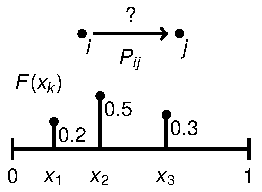
\includegraphics[width=0.69\linewidth]{%
        figures/tikz_line_right.pdf} % 
    \end{center}%\vspace{1cm}
       }
    \\
    \onslide<1->{   \vspace{-0.27cm} 
    Probability of connection a \myul{constant} $P_{ij}$,
    %\vspace{0.05cm}

    \begin{align*}
      P_{ij} = c
    \end{align*}
}
    &&

       \onslide<5->{\vspace{-0.27cm}
    Probability of connection a \myul{random variable} $P_{ij}$,
    \vspace{0.01cm}
    
    \begin{align*}
      \mathbf{Prob}(P_{ij}=x_k) = F(x_k)
    \end{align*}}	

    \\

        \onslide<2->{\vspace{-0.88cm}
    \textbf{Overall connection probability}
    \vspace{0.12cm}
    
    \begin{align*}
      \mu = P_{ij} = c
    \end{align*}}


    &&
    \onslide<6->{\vspace{-0.88cm}
    \textbf{Overall connection probability}
    \vspace{-0.08cm}
    
    \begin{align*}
      \mu = \sum_{k=1}^m F(x_k) x_k
    \end{align*}}
    
    \\
    \onslide<3->{\vspace{-0.8cm}
    \textbf{Bidirectional connection}
    \vspace{0.12cm}
    
    \begin{align*}
      P_{\text{bidir}} = P_{ij} P_{ji} = c^2
    \end{align*}	}

    &&
    \onslide<7->{\vspace{-0.8cm}
    \textbf{Bidirectional connection}
    \vspace{-0.08cm}

       \only<7-8>{\vspace{0.18cm}
    \begin{align*}
      P_{\text{bidir}} = \text{?} %\label{eq:TT}
    \end{align*}}
       \only<9-10>{
    \begin{align*}
      P_{\text{bidir}} = \sum_{k=1}^m \sum_{l=1}^m F(x_k) x_k \only<9>{F(x_l | x_k)}\only<10>{\myul[red]{F(x_l | x_k)}} x_l %\label{eq:TT}
    \end{align*}}}
    
  \end{tabular}

  
  % \source{\cite{Hoffmann2017}}
  
\end{frame}




\begin{frame}{}

    % 
    \begin{columns}
      % 
      \begin{column}{.5\textwidth}
        \minipage[c][0.85\textheight][s]{\columnwidth}

        \onslide<2->
        \begin{align*}
          P_{\text{bidir}} &= \sum_{k=1}^m \sum_{l=1}^m F(x_k) x_k F(x_l | x_k) x_l \\ &= \sum_{k=1}^m F(x_k) x_k^2 .
\end{align*}


\onslide<3->
\textit{Relative overrepresentation} $\varrho$ is the fraction

\begin{align*}
  \varrho = \frac{P_{\text{bidir}}}{\mu^2} = \frac{\sum_{k=1}^m F(x_k) x_k^2 }{\left(\sum_{k=1}^m F(x_k) x_k\right)^2}.
\end{align*}

\onslide<4->
By Jensen's inequality,

\begin{align*}
  \left(\sum_{k=1}^m F(x_k) x_k\right)^2 \leq \sum_{k=1}^m F(x_k) x_k^2  \quad \text{and thus} \quad \varrho \geq 1.
\end{align*}	

        
        \endminipage      
      \end{column}
      % 
      \begin{column}{.5\textwidth}
        \onslide<1->
        \minipage[c][0.85\textheight][s]{\columnwidth}

        \onslide<1->\begin{align*}
  F(x_l | x_k) = \begin{cases} 1 & \text{if $l = k$} \\ 0 & \text{otherwise.} \end{cases}
        \end{align*}


        
        \begin{figure}
          \centering
          \includegraphics[width=0.85\textwidth]{%
          /home/fh/sci/rsc/nrnd_pairs/pub/arxiv_16/figures/two_point_network/two_point_network.pdf} %
      \end{figure}

      \vspace{1.25cm}
        
        \endminipage
        
        
      \end{column}
    \end{columns}
    \onslide<1>\source{\normalsize \cite{Hoffmann2017}}
    
  \end{frame}

%   \begin{frame}
  
% \begin{align*}
%   F(x_l | x_k) = \begin{cases} 1 & \text{if $l = k$} \\ 0 & \text{otherwise.} \end{cases}
% \end{align*}
% Then


% \vspace{0.4cm}

% \textit{Relative overrepresentation} $\varrho$ is the fraction

% \begin{align*}
%   \varrho = \frac{P_{\text{bidir}}}{\mu^2} = \frac{\sum_{k=1}^m F(x_k) x_k^2 }{\left(\sum_{k=1}^m F(x_k) x_k\right)^2}.
% \end{align*}
% By Jensen's inequality,

% \begin{align*}
%   \left(\sum_{k=1}^m F(x_k) x_k\right)^2 \leq \sum_{k=1}^m F(x_k) x_k^2  \quad \text{and thus} \quad \varrho \geq 1.
% \end{align*}	
% %% If and only if $m > 1$, that is when the probability distribution of connection probabilities is non-degenerate, strict inequality in (2) holds.  

% \source{\normalsize \cite{Hoffmann2017}}
% \end{frame}


  \begin{frame}{}

    \begin{figure}
    \centering
    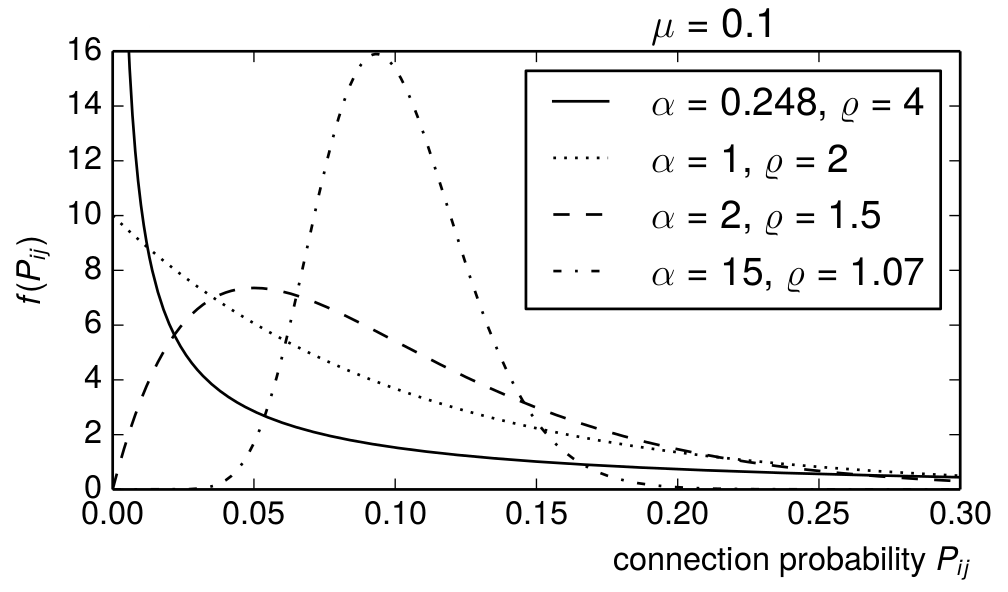
\includegraphics[width=0.8\textwidth]{%
      figures/nrnd_gamma.png} %
  \end{figure}

  \vspace{0.2cm}

  \begin{itemize}[leftmargin=1.3cm]
    \large
    \itemsep9pt
  \item[--]<2-> multiple neuron properties together can cause strong overrepresentation
  \item[--]<3> example: higher connection probability in functionally
\\    related cells \parencite{Lee2016a}

       
  \end{itemize}

  \vspace{0.4cm}
  
  

  \source{\normalsize \cite{Hoffmann2017}}
  
\end{frame}






\begin{frame}{Three neuron motifs}

  \begin{figure}
    \centering
    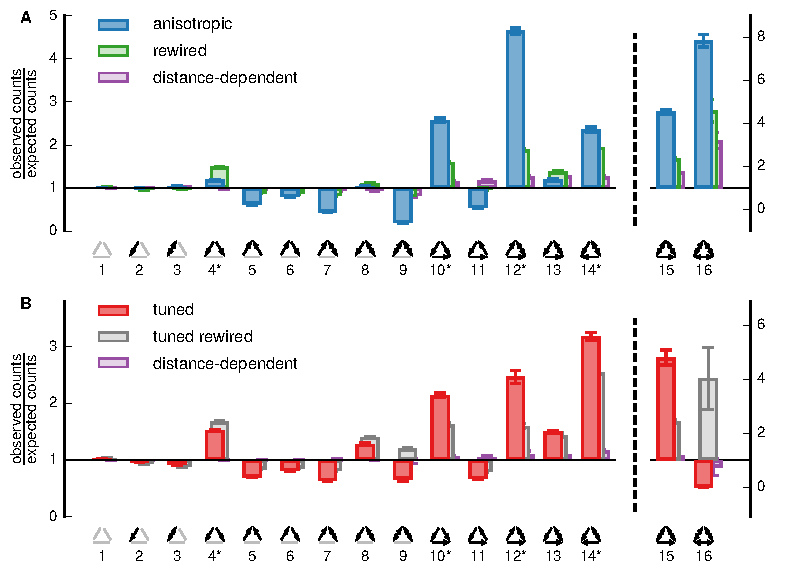
\includegraphics[width=\textwidth]{%
      figures/three_motifs_3x1.pdf} %
  \end{figure}
  

  % \source{Hoffmann \& Rotter, in prep.}
  
  
\end{frame}

\begin{frame}{Robust nonrandom connectivity patterns}
  % 
  \begin{columns}
    % 
    \begin{column}{.45\textwidth}
      \minipage[c][0.75\textheight][s]{\columnwidth}
      
      \begin{figure}
        \centering
        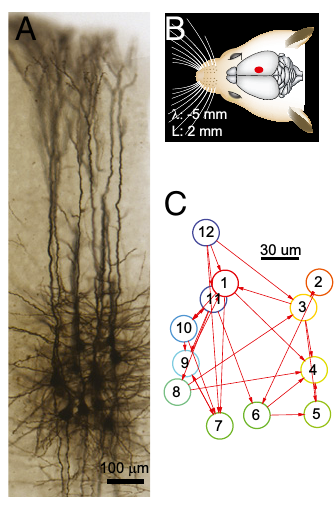
\includegraphics[width=\textwidth]{%
          figures/Perin2011_Fig1ABC.png} %
      \end{figure}
      

      
      \endminipage      
    \end{column}
    % 
    \begin{column}{.55\textwidth}


      \vspace{-0.2cm}
      
      \begin{figure}
        \centering
        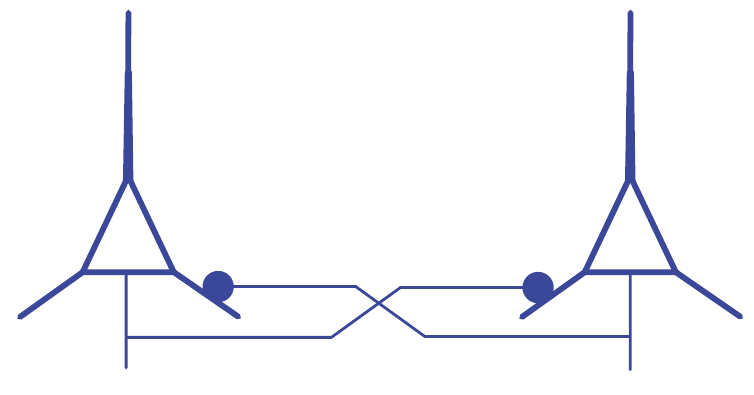
\includegraphics[width=0.525\textwidth]{%
          figures/two_neuron.png} %
      \end{figure}

      \vfill
      

      \begin{figure}
        \centering
        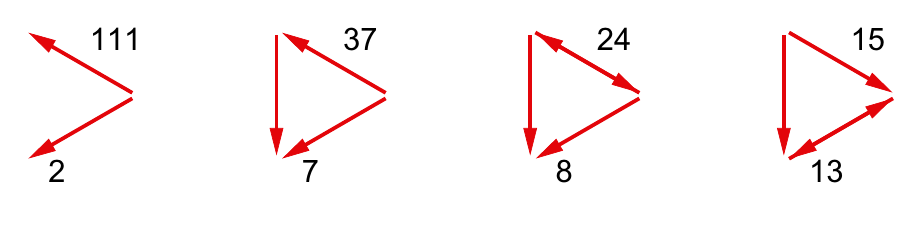
\includegraphics[width=\textwidth]{%
        figures/Perin2011_FigS2_custom.png} %
      \end{figure}

      \vfill
      

      \begin{figure}
        \centering
        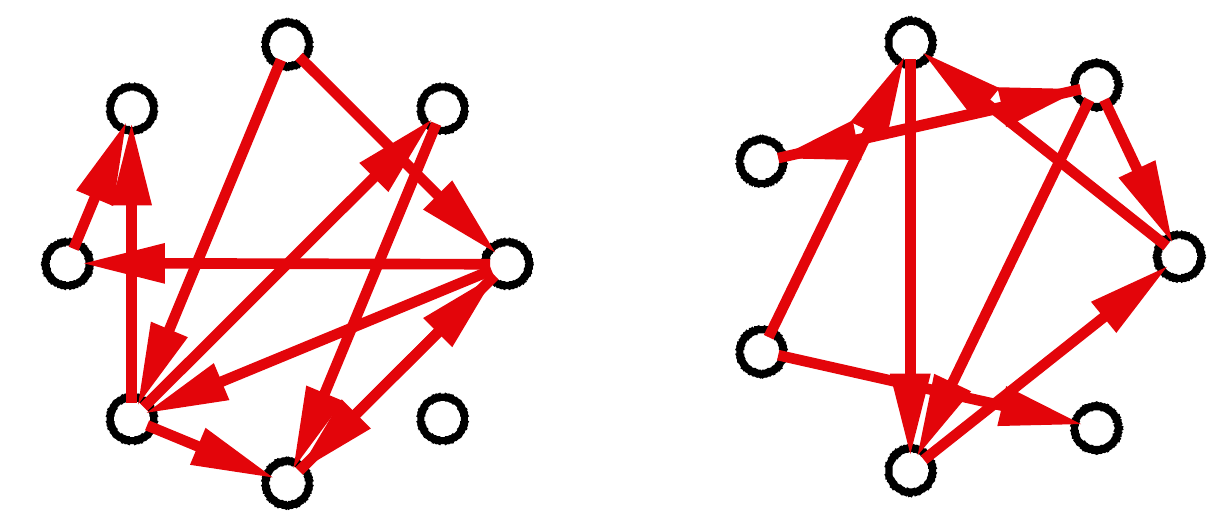
\includegraphics[width=0.7\textwidth]{%
          figures/clust_all.png} %
      \end{figure}
      
      \vfill

      
    \end{column}
  \end{columns}

  \source{\cite{Perin2011, Song2005, Markram1997, Miner2016, Gal2017,
      Vegue2017}}

  \pnote{
    
  }
  
\end{frame}



\begin{frame}{Connection counts in neuron clusters}

  \only<1>{
  \begin{figure}
    \centering
    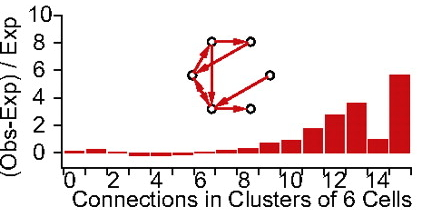
\includegraphics[width=0.85\textwidth]{%
      figures/perin_select6.png} %
  \end{figure}}
  

  \only<2>{
  \begin{figure}
    \centering
    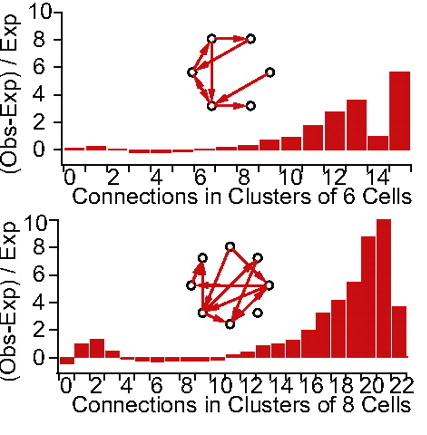
\includegraphics[width=0.625\textwidth]{%
      figures/perin_select2.png} %
  \end{figure}}

  \onslide<1-2>{\source{\cite{Perin2011}}}
  
\end{frame}



\begin{frame}{Connection counts in neuron clusters}

  \only<1>{
  \begin{figure}
    \centering
    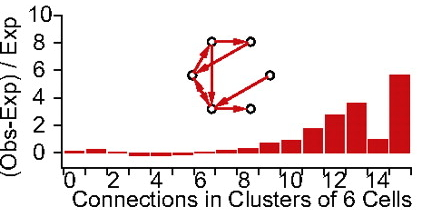
\includegraphics[width=0.625\textwidth]{%
      figures/perin_select6.png} %
  \end{figure}}


  \begin{figure}
    \centering
    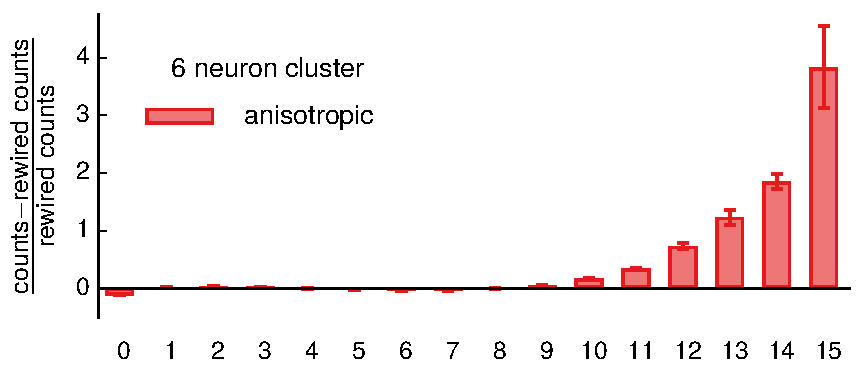
\includegraphics[width=0.875\textwidth]{%
    figures/fig5C_6cluster_counts.pdf} %
  \end{figure} 
  
\end{frame}


\begin{frame}{Connection counts in neuron clusters}

  \vspace{0.1cm}
    \only<1>{
  \begin{figure}
    \centering
    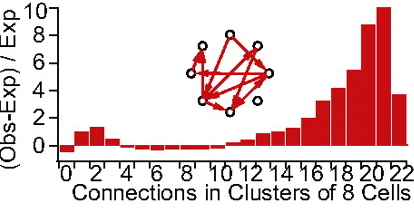
\includegraphics[width=0.625\textwidth]{%
      figures/8cluster_perin.png} %
  \end{figure}}

  \vspace{-0.5cm}

  \begin{figure}
    \centering
    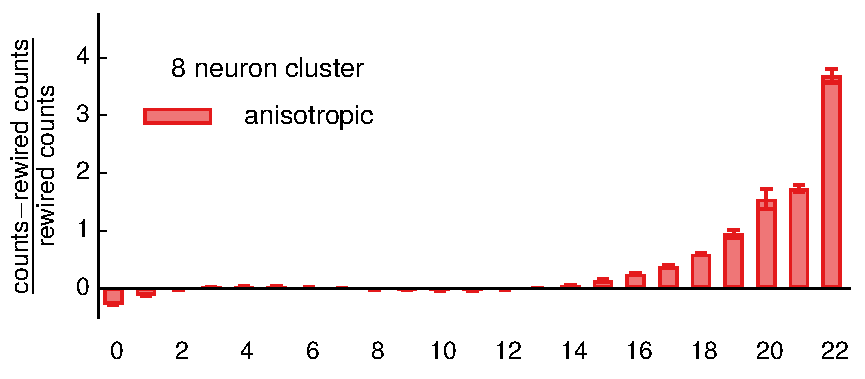
\includegraphics[width=0.875\textwidth]{%
    figures/fig5E_8cluster_counts.pdf} %
  \end{figure} 
  
\end{frame}

\begin{frame}{Common inputs statistics}

  \begin{figure}
    \centering
    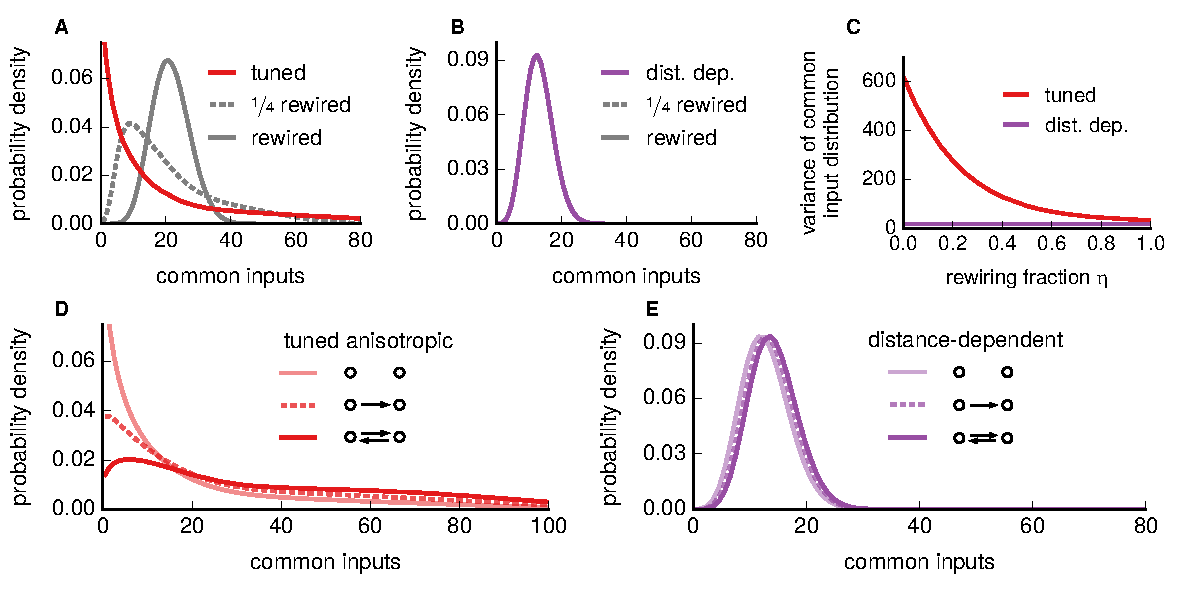
\includegraphics[width=\textwidth]{%
      figures/fig6.pdf} %
  \end{figure}  
  
\end{frame}


\begin{frame}{Summary 1-1}

  \large\textbf{Model}
  
  \begin{itemize}[leftmargin=0.6cm]
    \large
    \itemsep6pt
  \item[--] anisotropy in spatial connectivity as a result of
    stereotypical axon and dendrite morphology
  \item[--] anisotropic network as a simple model to test how
    anisotropy in spatial connectivity impacts network connectivity
  \end{itemize}

  \vfill

  \large\textbf{Results}
  
  \begin{itemize}[leftmargin=0.6cm]
    \large
    \itemsep6pt
  \item[--] reciprocal connections are overrepresented but only
    due induced distance-dependency
  \item[--] various neuron properties (such as functional
    similarity) may compound with distance\--dependency to induce
    observed reciprocity in cortical circuits
    
  \end{itemize}


\end{frame}

\begin{frame}{Summary 1-2}

  \large\textbf{Results}
  
  \begin{itemize}[leftmargin=0.6cm]
    \large
    \itemsep6pt
  \item[--] specific three neuron motifs occur over- and
    underrepresented due to anisotropy matching data from
    cortical circuits
  \item[--] observed frequent occurrence of high connection counts in
    neuron groups as a direct result of anisotropy in spatial
    connectivity
    
  \end{itemize}

  \vfill
  
  \large\textbf{Predictions}
  
  \begin{itemize}[leftmargin=0.6cm]
    \large
    \itemsep6pt
  \item[--] anisotropic network model predicts broad distributions of common
    inputs for neuron pairs
  \item[--] anisotropic network model predicts stronger sensitivity to
    connection type for common input distributions
  \end{itemize}  
  
\end{frame}


%% Synaptic lifetimes

\begin{frame}{The dynamic connectome}

  \only<1>{  \Large
    At the synapse level, brain circuitry is constantly making new connections and abolishing old ones \nocite{Rumpel2016}

    \vspace{0.4cm}}
  \only<2->{\vspace{-0.6cm}}
  
  \begin{figure}
    \centering
    \includegraphics<1>[height=0.5\textheight]{%
      figures/Loewenstein2015_Fig1A.png} %
    \includegraphics<2->[height=0.5\textheight]{%
      figures/Loewenstein2015_Fig1B.png} %
    \includegraphics<2->[height=0.5\textheight]{%
      figures/Loewenstein2015_Fig2A.png} %
  \end{figure}

  \only<2->{\vspace{0.3cm}
    \begin{center}
      \minipage[c][0.14\textheight][s]{0.9\textwidth}
      
      \Large%
      Survival probability of $\varrho(t) = (t+1)^{-\gamma}$ with $\gamma \approx 1.4$,\\[10pt]
      equivalently lifetime distribution of
      $f(t) = \gamma (t+1)^{-(\gamma+1)}$
      \endminipage      

    \end{center}}
  
  \source{\cite{Loewenstein2015}}

  \pnote{

    - chronic two-photon imaging through\\
    a cranial window
    
    - auditory cortex in mice (expressing GFP\\
    in a subset of pyramidal neurons)

    Figure: 4 Days apart!

    - image spines from 8 neurons\\
    spine count almost constant!
    
    
  }
  
\end{frame}



\begin{frame}{Synapse dynamics in self-organizing recurrent networks}
  
  % 
  \begin{columns}
    % 
    \begin{column}{.425\textwidth}
      \minipage[c][0.55\textheight][s]{\columnwidth}

      Power law synaptic lifetime distribution -- \cite{Zheng2013}

      \vfill
      
      \onslide<2-> Extension to leaky integrate-and-fire neuron --
      \cite{Miner2016}

      \vfill

      \onslide<3> Synapse dynamics under inclusion of iSTDP --
      \cite{Kleberg2018a}

      \vspace{0.8cm}
      
      \endminipage      
    \end{column}
    % 
    \begin{column}{.575\textwidth}
      \minipage[c][0.6\textheight][s]{\columnwidth}
      \onslide<1->
      \begin{figure}
        \centering
        \includegraphics<1>[width=\textwidth]{%
          figures/Zheng2013_custom2.png} %
        \includegraphics<2>[width=\textwidth]{%
          figures/Miner2016_Fig6.png} %
        \includegraphics<3>[width=.55\textwidth]{%
          figures/Kleberg2018_custom2.png} %        

      \end{figure}

      \endminipage
      
    \end{column}
  \end{columns}
  

  \only<1>{\source{\cite{Zheng2013}}}
  \only<2>{\source{\cite{Miner2016}}}
  \only<3>{\source{\cite{Kleberg2018a}}}

  
\end{frame}


\begin{frame}{Lifetimes in the self-organizing recurrent network}

  \vspace{0.55cm}
  \vspace{-0.4cm}

  \begin{figure}
    \centering
    \includegraphics<1>[width=0.925\textwidth]{%
      /home/fh/sci/lab/syn_lt/sorn_model/set_02/img/fpt_lfsn-long_green.png}
  \end{figure}

  \vspace{-0.2cm}

  \Large
  \begin{align*}
    D = \text{LTD--LTP balance}
  \end{align*}

  
  \pnote{
    
    Does not depend on

    -- network size

    -- membrane noise levels

    -- exact synaptic scaling implementation
    
  }
  
\end{frame}



\begin{frame}{Lifetimes modelled by a stochastic process}

  \vspace{0.55cm}

  \large Kesten process (\cite{Kesten1973, Statman2014})

  \begin{align*}
  X_{n+1} = a_n X_n + b_n
  \end{align*}

  as a model for synapse dynamics

  \vspace{0.3cm}

  \begin{figure}
    \centering
    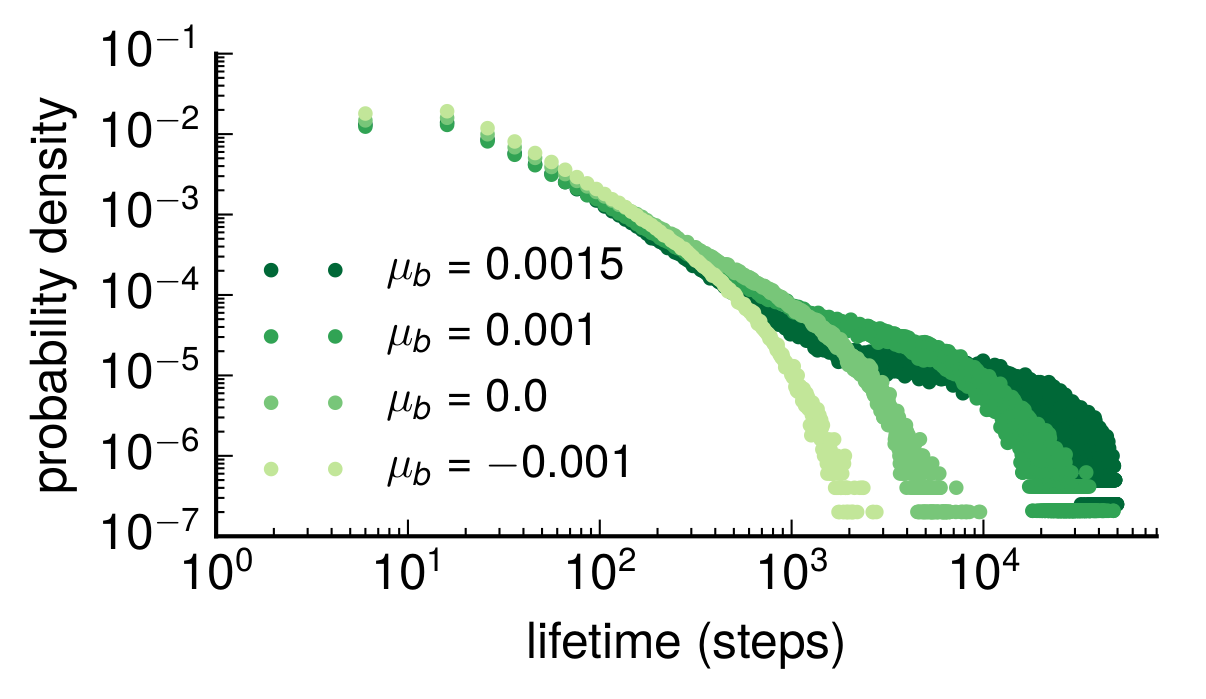
\includegraphics[width=0.85\textwidth]{%
      figures/lft1.png} %
  \end{figure}
  
 
\end{frame}





%% Summary / Discussion


\begin{frame}{Acknowledgements}
  % 
  \begin{columns}
    % 
    \begin{column}{.425\textwidth}
      \minipage[c][0.65\textheight][s]{\columnwidth}
      
      
      
      \endminipage      
    \end{column}
    % 
    \begin{column}{.575\textwidth}
      \onslide<1->
      
      
    \end{column}
  \end{columns}
  
\end{frame}


\begin{frame}[t]{References \hspace{3.25cm} }

  \begin{multicols}{2}
    \printbibliography
  \end{multicols}
  \vspace{0.25cm}
  %% \begin{center}
  %%   \Large
  %%   \textit{Thank you!}
  %% \end{center}

  \pnote {

  }
  
\end{frame}


%% Overflow
% \begin{frame}{Overflow -- Rewiring parameters}
  
  \begin{figure}
    \centering
    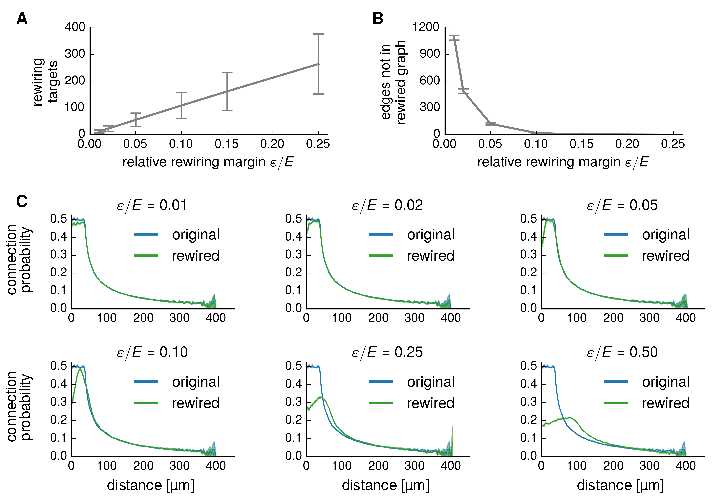
\includegraphics[width=\textwidth]{%
    figures/SI_rew.pdf} %
  \end{figure}
  
\end{frame}


\begin{frame}{Overflow -- Degree distributions}

  \begin{figure}
    \centering
    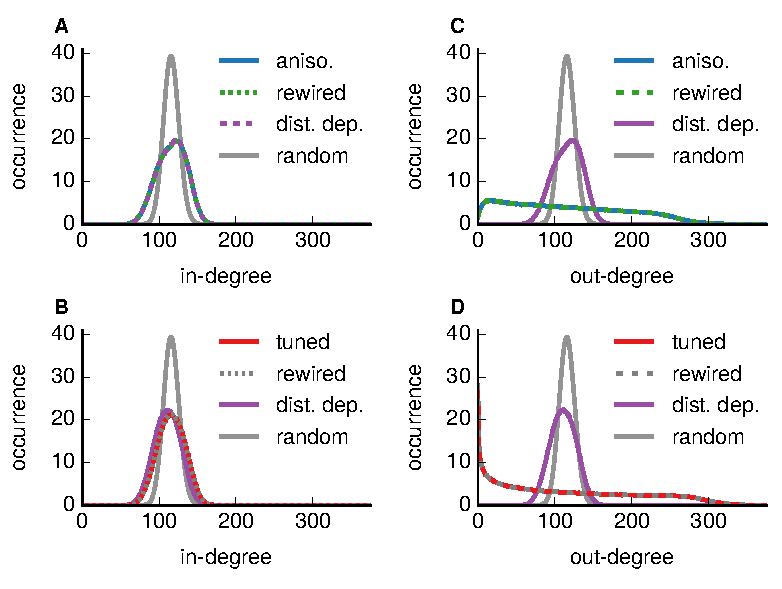
\includegraphics[width=0.9\textwidth]{%
    figures/io_degrees_2x2_alt.pdf} %
  \end{figure}
  
  
\end{frame}



\end{document}
















